%TeX

\section{Finding the flag}

\begin{frame}{A quick recap\ldots}
    \begin{columns}
        \column{0.5\textwidth}
        \begin{itemize}
            \item<1-> We have an x86 boot sector that's asking us for the flag
            \item<2-> The flag is clearly in the boot sector SOMEWHERE\ldots
            \begin{itemize}
                \item<3-> \ldots but not in plaintext, because this is a 400
                          point challenge and that would be too easy
            \end{itemize}
            \item<4-> So, where is it?
        \end{itemize}
        \column{0.5\textwidth}
        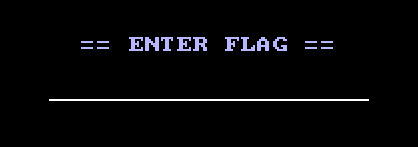
\includegraphics[width=\textwidth]{enter-flag}
    \end{columns}
\end{frame}

\begin{frame}{Reversing the boot sector}
    \begin{columns}
        \column{0.5\textwidth}
        \begin{itemize}
            \item<1-> Open the file in your favorite disassembler (e.g. IDA);
                      rebase at \texttt{0x7c00}
            \item<2-> We can visally pick out three sections:
            \begin{itemize}
                \item<2-> Init code (responsible for the protected
                          mode transition)
                \item<2-> Display code (identifiable by a large number of
                          \texttt{int} instructions)
                \item<2-> Some other code that uses Intel SSE2 instructions
            \end{itemize}
        \end{itemize}
        \column{0.5\textwidth}
        \begin{tikzpicture}
            \only<1> {\node (cfg) {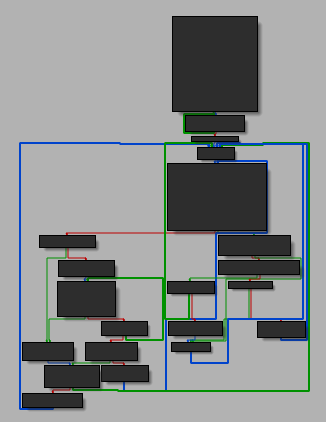
\includegraphics[width=\textwidth]{cfg}};}
            \uncover<2-> {\node (cfga) 
                {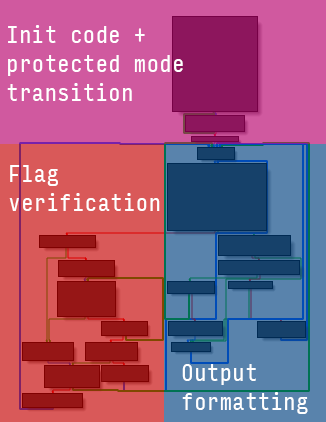
\includegraphics[width=\textwidth]{cfg-annotated}};}
        \end{tikzpicture}
    \end{columns}
\end{frame}

\begin{frame}{First leads}
    \begin{itemize}
        \item<1-> The program asks you to enter 20 characters, and immediately
                  breaks out if the first 4 characters aren't 'flag'
        \item<2-> We can verify this in a debugger after eyeballing the code

        \begin{center}
            \uncover<3-> {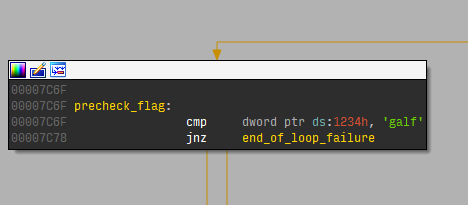
\includegraphics[width=0.7\textwidth]{flag-precheck}}
        \end{center}
    \end{itemize}
\end{frame}

\begin{frame}{Suddenly, SSE2 instructions}
    \framesubtitle{``My Intel CPU can do {\em that?}''}
    The author of the challenge decided to use a bunch of obscure x86 SSE2
    instructions to force us to trawl through Intel documentation

    \begin{itemize}
        \item<2-> movaps\uncover<3->{: Moves to/from/between XMM registers}
        \item<2-> andps\uncover<3->{: Performs bitwise AND between XMM
                                      registers}
        \item<2-> pshufd\uncover<3->{: Shuffles 32-bit words in XMM registers}
        \item<2-> psadbw\uncover<3->{: Sums absolute values of differences
                                       between bytes (it's as crazy as it
                                       sounds)}
    \end{itemize}

    \begin{block}{Note}
        SSE2 instructions operate on XMM registers, which are 128 bits
        (16 bytes) wide.
    \end{block}
\end{frame}

\begin{comment}
% commented out for now, broke the flow of the presentation

\begin{frame}{As it turns out\ldots}
    \begin{itemize}
        \item<1-> The flag is hashed, (and this isn't a surprise\ldots{} why?)
            % because the hashed flag can be stored in the program without
            % storing the actual flag
        \item<2-> The hash algorithm is custom
        \item<3-> The custom hash algorithm is almost entirely implemented
                  using Intel AVX vector instructions
        \item<4-> Ugh\ldots
    \end{itemize}
\end{frame}

\begin{frame}{What typically goes into a hash function?}
    \framesubtitle{It's only sort of magic}
    \begin{itemize}
        \item<1-> Hash functions are usually defined as
                  $H(s, x) \rightarrow \{0, 1\}^\ell$, where $s$ is the 'seed',
                  $x$ is the message, and $\ell$ is some fixed number of bits
        \item<2-> The 'seed' is some public value used to initialize the hash
                  function's state
        \item<3-> Generally, there are a series of repeated 'reductions' meant
                  to take the message and perform some sort of irreversible
                  transform on it one block at a time
    \end{itemize}
    \pause \pause \pause
    \begin{block}{Example}
        For SHA256, $s$ is the fractional part of the cube roots of the first
        64 primes, $\ell = 256$, and the reductions involve a few non-linear
        functions (i.e. addition/XOR of multiple values, taking the majority of
        three bits, etc). The idea is that {\em you can't get the original
        message back once you start scrambling it.}
    \end{block}
\end{frame}

\begin{frame}{But, this is a CTF\ldots}
    \begin{itemize}
        \item<1-> They wouldn't hash the flag with a strong hash function and
                  expect us to break it
        \item<2-> The hash function has to fit in 512 bytes of x86 instructions
        \item<3-> So\ldots{} we can expect that we have to reverse engineer the
                  hash function to recover the flag
    \end{itemize}
\end{frame}
\end{comment}
